 \documentclass{beamer}

\usepackage[utf8]{inputenc}
\usepackage{graphicx}
\usetheme{Boadilla} % Beamer theme

\title{Licence Pro ADSILLH}
 
\subtitle{GNOME-Games / GNOME-Music}
 
\author{Groupe Games:\\ Pierre Antoine Rouby,\\ Gautier Delacour,\\
  David Tabarie,\\
  \vspace{0.8cm}
  Groupe Music:\\ Kevine Carsoule,\\ Adrien Darfeuille}

\date{Année 2017/2018}

% ce code permet d'afficher le sommaire à chaque section,
% en mettant en valeur la section courante (utile ?)
\AtBeginSection[]
{
  \begin{frame}
    \frametitle{Sommaire}
    \tableofcontents[currentsection]
  \end{frame}
}

\begin{document}
\frame{\titlepage}

\section{Le projet Gnome}
\begin{frame}
  \frametitle{Le projet Gnome}
    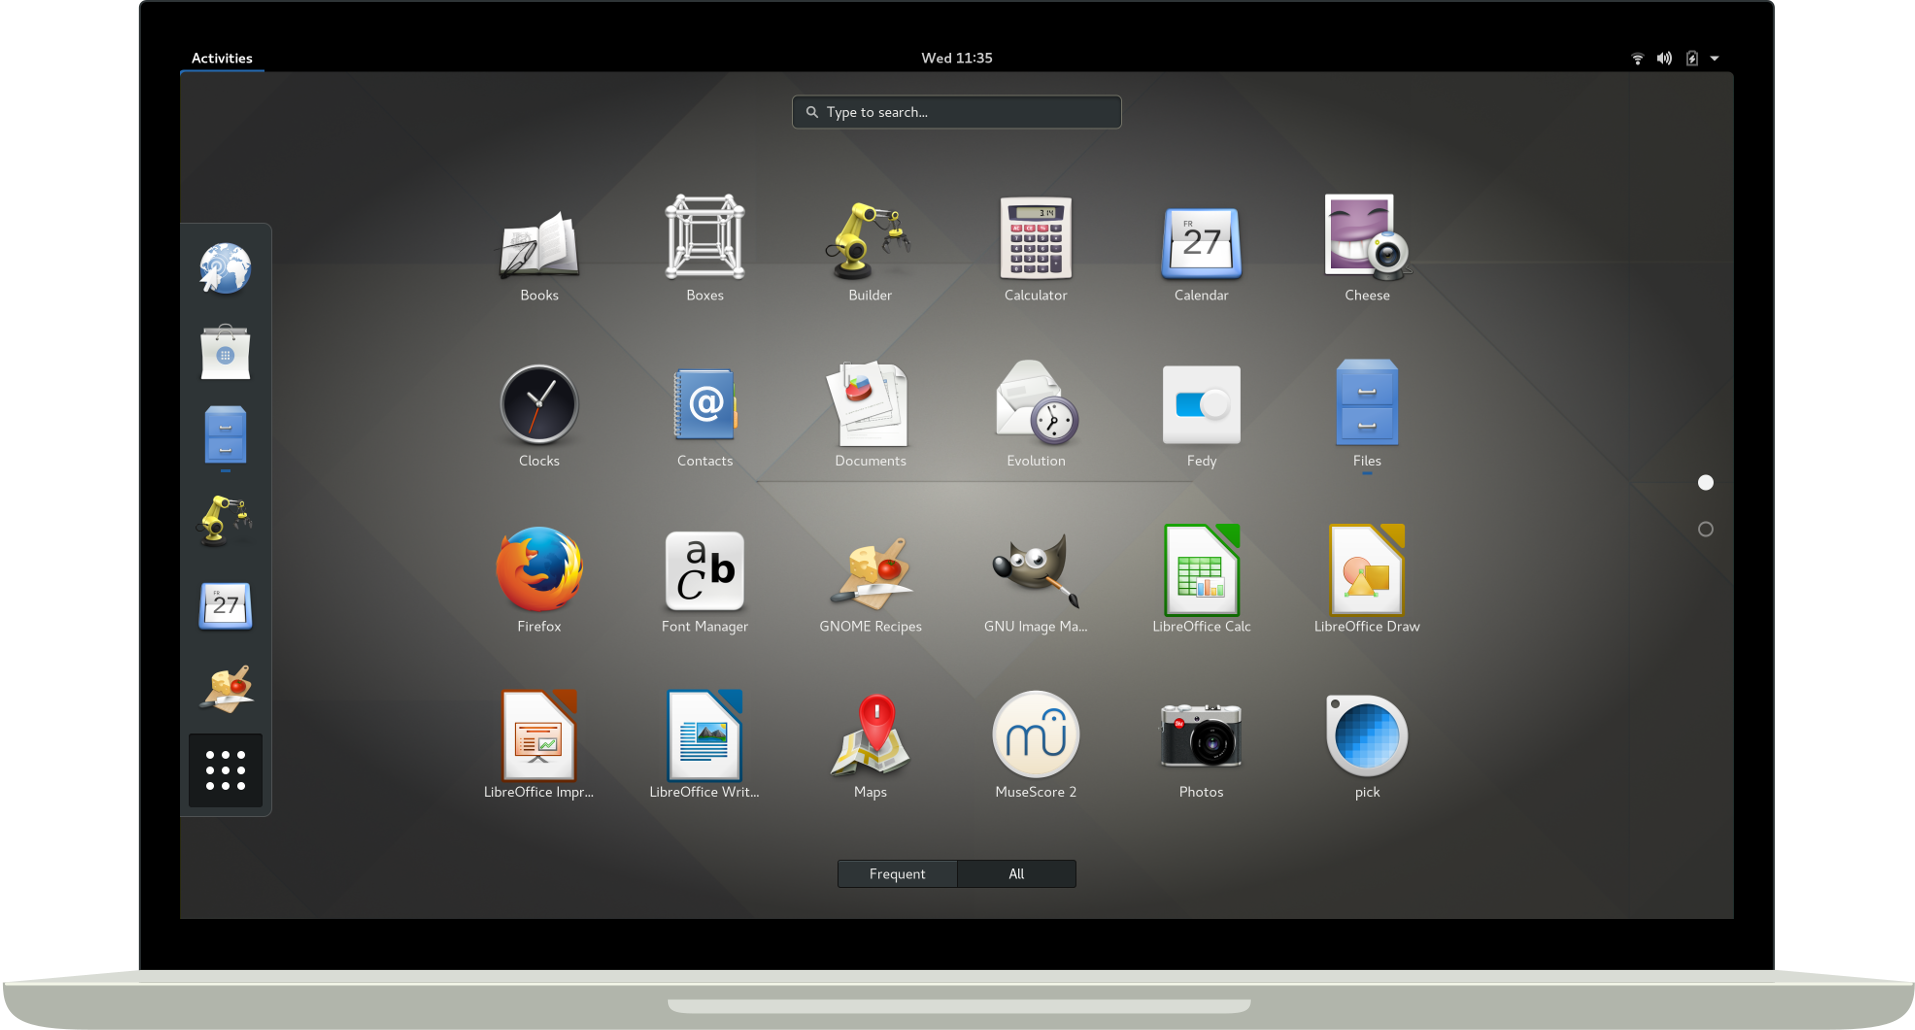
\includegraphics[scale=0.235]{images/GnomeScreen.png}
\end{frame}

\section{Le projet Gnome Games}
\begin{frame}
  \frametitle{GNOME Games}
  \includegraphics[scale=0.3]{images/screen-games.png}
\end{frame}

\subsection{Contributions effectués sur GNOME Games}
\begin{frame}
  \frametitle{Contributions effectués}
  \begin{itemize}
    \item Traçage d'un bug Pulseaudio
    \item Patch 1: Modifications du fichier 'HACKING'
    \item Patch 2: Modifications du fichier README.md
    \item Patch 3: Ajout d'un event 'retour au menu'
  \end{itemize}
\end{frame}

\subsection{Conclusion Games}
\begin{frame}
  \frametitle{Conclusion Games}
\end{frame}

\section{Le projet Gnome Music}
\begin{frame}
  \frametitle{Le projet Gnome Music}
\end{frame}

\subsection{Contributions effectués sur GNOME Music}
\subsection{Ce que vous avez fait}
\begin{frame}
  \frametitle{}
\end{frame}

\subsection{Conclusion Music}
\begin{frame}
  \frametitle{Conclusion Music}
\end{frame}

\end{document}
